\documentclass[11.5pt]{sig-alternate} % sets document style to sig-alternate
% packages
% typesetting
%\usepackage{dirtytalk} % typset quotations easier (\say{stuff})
\usepackage{hanging} % hanging paragraphs
\usepackage[defaultlines=3,all]{nowidow} % avoid widows
\usepackage[pdfpagelabels=false]{hyperref} % produce hypertext links, includes backref and nameref
\usepackage{xurl} % defines url linebreaks, loads url package
\usepackage{microtype}
%\usepackage[super]{nth} % easily create superscript ordinal numbers with \nth{x}
\usepackage{textcomp}
\newcommand{\texttildemid}{\raisebox{0.4ex}{\texttildelow}}
% layout
%\usepackage{enumitem} % control layout of itemize, enumerate, description
\usepackage{fancyhdr} % control page headers and footers
\usepackage{float} % improved interface for floating objects
%\usepackage{multicol} % intermix single and multiple column pages
% language
\usepackage[utf8]{inputenc} % accept different input encodings
\usepackage[english]{babel} % multilanguage support
% misc
\usepackage{graphicx} % builds upon graphics package, \includegraphics
%\usepackage{lastpage} % reference number of pages
%\usepackage{comment} % exclude portions of text (?)
\usepackage{xcolor} % color extensions
\usepackage[backend=biber, style=apa]{biblatex} % sophisticated bibliographies % necessary for HTML to display author info and date on abstract page
\usepackage{csquotes} % advanced quotations, makes biblatex happy
\usepackage{authblk} % support for footnote style author/affiliation
% tables and figures
\usepackage{tabularray}
%\usepackage{array} % extend array and tabular environments
\usepackage{caption} % customize captions in figures and tables (rotating captions, sideways captions, etc)
%\usepackage{cuted} % allow mixing of \onecolumn and \twocolumn on same page
\usepackage{multirow} % create tabular cells spanning multiple rows
%\usepackage{subfigure} % deprecated, support for manipulation of small figures
%\usepackage{tabularx} % extension of tabular with column designator "x", creates paragraph-like column whose width automatically expands
%\usepackage{wrapfig} % allows figures or tables to have text wrapped around them
%\usepackage{booktabs} % better rules
% dummy text
%\usepackage{blindtext} % blind text dummy text
%\usepackage{kantlipsum} % Kant style dummy text
\usepackage{lipsum} %lorem ipsum dummy text
% other helpful packages may be booktabs, longtable, longtabu, microtype

\pagestyle{fancy} % sets pagestyle to fancy for fancy headers and footers

% header and footer
% modern way to set header image
\renewcommand{\headrulewidth}{0pt} % defines thickness of line under header
\renewcommand{\footrulewidth}{0pt} % defines thickness of line above header
\setlength\headheight{80.0pt} % sets height between top margin and header image, effectively moves page contents down
\addtolength{\textheight}{-80.0pt} % seems to affect the lower height. maybe only works properly if footer numbers enabled?
\fancyhf{}
\fancyhead[CE, CO]{
\includegraphics[width=\textwidth]{headerImage.png}}
% footer
%\fancyfoot[LE,LO]{Article Title Here \\ DOI: }% left footer article title and doi
%\fancyfoot[CE,CO]{{}} % center footer empty
%\fancyfoot[RE,RO]{\thepage} % right footer page numbers
%\pagenumbering{arabic} % arabic (1, 2, 3) numbering in footer

\hypersetup{colorlinks=true,urlcolor=blue} % sets link color to blue
\urlstyle{same} % sets url typeface to same as rest of text

% set caption and figure to italics, label bold, left align captions, does not transfer to HTML
\captionsetup{labelfont=bf, font={large, it}, justification=raggedright, singlelinecheck=false}
\renewcommand\theContinuedFloat{\alph{ContinuedFloat}}

%this next bit is confusing, but essentially changes the width of the abstract. Seems to have been copied from this https://tex.stackexchange.com/questions/151583/how-to-adjust-the-width-of-abstract
\let\oldabstract\abstract
\let\oldendabstract\endabstract
\makeatletter %changes @ catcode to enable modification (in parsep)
\renewenvironment{abstract} %alters the abstract environment
{\renewenvironment{quotation}%
               {\list{}{\addtolength{\leftmargin}{1em} % change this value to add or remove length to the the default ?
                        \listparindent 1.5em%
                        \itemindent    \listparindent%
                        \rightmargin   \leftmargin%
                        \parsep        \z@ \@plus\p@}%
                \item\relax}%
               {\endlist}%
\oldabstract}
{\oldendabstract}
\makeatother %changes @ catcode to disable modification

% checks
% italics -
% links -
% dashes -
% tildes -
\begin{document}

\title{Making 3D Laser Cut Stratigraphic Audio-responsive Tactile Templates}

\author[1]{\large \color{blue}Michael A. Kolitsky}

\affil[1]{nextgenEmedia}

\toappear{}
%% ABSTRACT
\maketitle
\begin{@twocolumnfalse} 
\begin{abstract}
\item 
\textit{The geologic method of stratigraphy which studies the structure of the earth by making layers was employed with 3D laser cutting techniques to make more easily defined tactile regions in templates of cells, tissues and anatomic regions containing muscles and bones. Templates were made audio responsive by hand-drilling a small hole in a template and filling that hole with conductive electric paint. A finger touch to the template top side now carries a charge similar to an electric circuit to the template bottom side resting on the surface of an iPad or iPad Pro where an audio button produces audio describing what structure was touched on the upper surface. Templates made using laser cutting start with 3 mm width acrylic sheets and use svg (scalable vector graphics) files made from line drawings of cells or tissues or anatomic sections. Some variation in height between acrylic pieces lying next to each other can utilize 3D laser cut veneer (thin 1mm width wood) placed underneath one laser cut acrylic piece to more easily produce a tactile difference between two acrylic pieces lying close to each other such as with a muscle and a bone. Examples of 3D laser cut audio-responsive templates include structures associated with a chicken egg and the organelles of a typical cell made from line drawings from the TAEVIS collection originally designed for making raised line graphics from swell paper. Also included are examples made from transverse sections of a human cadaver contained in the National Library of Medicine “Visible Human” project.}
\\ \\
Keywords: 3D laser cutting, audio-enriched tactile templates, electric paint
\end{abstract}
\end{@twocolumnfalse}

%% AUTHOR INFORMATION

\textbf{*Corresponding Author,Michael A. Kolitsky }\\
\href{mailto: mkolitsky@snip.net}{(mkolitsky@snip.net)} \\
\textit{Submitted  November 16th, 2018}\\
\textit{Accepted January 2nd, 2018} \\
\textit{Published online April 5th, 2019} \\
\textit{DOI:10.14448/jsesd.11.0006} \\
\pagebreak
\clearpage
\begin{large}

\section*{INTRODUCTION}

If being able to learn is dependent upon building a mental image of what is to be studied, one can begin to sense the challenges presented to blind students in their study of material that can only be seen with the light or electron microscope or observed in a virtual or interactive digital display.  It is to this end that the field of tactile graphics has emerged to explore and assist in providing touch-enhanced learning opportunities for students with visual impairments.     

One traditional approach to creating tactile graphics to assist in building mental images through touch involves the use of raised line graphic paper.  This type of paper is also called capsule or swell paper because the paper when heated swells where black or dark lines are present on the paper.  The swollen lines or regions can be designed from diagrams or line drawings of material to be studied and Braille can also be added in raised fashion for identifying regions for study on a raised line graphic.  

In addition to raised line graphics, audio enrichment methods have also been explored by using 3D prints made with electrically conductive graphene-based filament that can carry the electrical activity of a finger touch to the surface of an iPad causing an audio button to fire providing information about the structure or region being touched. (1)  Although 3D printing is becoming more popular in schools and university settings, the use of graphene filament along with traditional non-conductive filament is more complicated because it requires a 3D printer that can print with two filament extruders at the same time or a two-step process to 3D print the conductive and non-conductive portions separately and then combine them to make the audio-enriched template.  

The challenge of making a 3D printed or a 3D laser cut template audio responsive to a fingertip touch is to create a way for the electrical activity of a finger touch to reach the surface of an iPad or iPad Pro audio button so that it can fire and read the recorded audio.  As will be discussed in this report, one new approach is to drill a hole into the 3D print or 3D laser cut template and fill it with conductive electric paint (2) that now serves like an electrical circuit to carry the finger electric charge down to the audio button on the iPad or iPad Pro screen surface.  And in addition, this report will also show how the use of a 3D laser cutter can make highly tactile templates that expand the options for creating ways to study STEM (science, technology, engineering and mathematics) areas that prove more challenging for students with vision impairments.        

The introduction of a 3D laser cutter for the consumer market in mid-2018 by Glowforge (3) made possible the exploration of how 3D laser cut tactile templates could be designed for learning in the STEM field.  3D laser cut templates were made with 3 mm thick acrylic sheets using svg (scalable vector graphics) files of line graphics from two sources.  High quality line diagrams from the TAEVIS (Tactile Access to Education for Visually Impaired Students) collection owned by Independence Science (4) which were designed for making raised line STEM graphics from swell paper were used as one source and digital images of transverse sections of a human cadaver from the National Library of Medicine “Visible Human” project (5) served as the second source.  The tactile templates were designed using a stratigraphic approach similar to the geologic study of the layers of the earth so that svg files for cells and tissues and also for the muscles and bones in the anatomic sections consisted of layers which increased the tactile definition of the regions to be studied and identified.  The increase in tactile definition, however, worked against permitting a fingertip touch electrical charge from reaching the surface of an iPad or iPad Pro showing images containing audio buttons.  This problem was solved by hand-drilling small holes one mm in diameter through the acrylic layers and filling them with conductive electric paint (2) which is normally used to make electronic circuits.  Now any region or layer on the stratigraphic surface can have a small hole hand-drilled into it and filled with conductive paint so that a fingertip touch can carry an electric charge from the surface of a template to the underneath area and when the underneath area is sitting on an iPad or iPad Pro surface with an audio button placed beneath the drilled hole, the transmitted electric charge will cause the audio button to fire just as if a finger touched the button directly.  This type of “at a distance” delivery of an electric charge from a fingertip touch on the surface of a template also means that the finger touch does not have to be directly over the drilled hole filled with electric paint.  The electric paint can be spread over a wider area and then a touch to any region of the electric paint will form a complete circuit carrying the electric charge to the audio button beneath the drilled hole causing the button to fire and produce an audio response to a single touch.  Other types of material can also be used for laser cutting such as the thinner veneer (about one mm thick) made from wood which can be laser cut at the same size of muscles and bones in a 2D anatomic section and then glued to the underneath portion of the 3 mm width acrylic to serve as another way to raise the acrylic above the surrounding material.  An entire bone or muscle can then have one or more thin veneer pieces glued to the underneath acrylic thereby raising the bone or muscle above the surrounding structures to better clarify the tactile definition of the structure compared to its surroundings.  A drilled hole filled with electric paint then connects that raised acrylic muscle or bone in its more easily defined tactile state to the audio button on an iPad or iPad Pro.

The focus of this report is twofold.  First, it will be shown how 3D laser cutting techniques can be applied to the production of highly tactile regions in a 2-dimensional STEM template and second, it will be further demonstrated how these thicker highly tactile regions can be made audio responsive through the use of small hand-drilled holes containing conductive “electric paint” when laid atop an iPad or iPad Pro with audio buttons underneath the “electric paint” regions.  It should also be noted that although this report focuses on tactile templates made from acrylic on a 3D laser cutter, the 3D STEM tactile templates made using 3D printing methodology (6) can also have small holes drilled into them and filled with conductive electric paint to provide a touch enabled audio response.  This opens up the opportunity to modify many 3D printed tactile templates to become audio responsive and indicates that further work must be done to determine where it is best to employ 3D printing or 3D laser cutting or even raised line swell paper for the production of audio-enriched tactile templates using electric paint.

\section*{METHODS}
 
\subsection*{3D laser cutting}

Since the introduction of Glowforge 3D laser cutters (3) in mid-2018, they have been used to make maps and artistic works using stratigraphic methods (7) but no examples have been found of using stratigraphic methods to make tactile templates for study of cells, tissues and human anatomic sections.  Stratigraphy can easily emphasize differences that exist in 2D sections of structures such as organelles in cells as well as muscles and bones in anatomic sections thereby supporting learning through tactile means.  3D laser cutting requires the production of scalable vector graphics files (svg files) and for this study, the program titled “Super Vectorizer 2” (8) was used on a Mac operating system.  In the “Super Vectorizer 2” program, the “line” option was used with “skeletonization” selected to produce svg files comprised of lines representing where the Glowforge laser should cut through the acrylic plastic sheet placed in the laser cutter.  Acrylic plastic sheets (9) of various colors and sizes were purchased from Glowforge and these acrylic sheets were guaranteed to meet safety standards in case any fumes from the laser cutter were not vented properly.  Adobe Photoshop was used to modify 2D color images from the National Library of Medicine “Visible Human” project (5) so that muscles and bones were outlined in black to produce svg line drawings that could then be laser cut.  Other svg files of cell structures and organelles were produced from line drawings made from the TAEVIS collection of images (4) normally used for the production of raised line graphics with swell paper.

\subsubsection*{Conductive paint}

3D laser cutting can produce a many layered stratigraphic template that can be laid atop an iPad or iPad Pro for the generation of audio from the graphics on the iPad or iPad Pro surface.  But acrylic plastic sheets that are 3 mm thick are not conductive, i.e., they do not pass a finger touch electrical activity through them to an audio button on an iPad or iPad Pro screen surface.  Small holes, however, drilled into the acrylic plastic template can be filled with “electric paint” from “Bare Conductive”. (2)  The electric paint now forms a conductive path from the template surface to the iPad or iPad Pro screen so that when a finger now touches the conductive paint on the tactile surface of the template, the electric charge of the finger touch will set off an audio button on the iPad or iPad Pro surface.
     
This method of filling small holes drilled into a template with conductive electric paint was first observed using a 3D print rather than a 3D laser cut template and an example 3D print of a transverse section of the human head with hand drilled holes can be seen in Figure 1.
      
In Figure 1 below,note in the above 3D print the tiny 1 mm diameter holes made with the hand drill located just below the 3D print and compare where the drilled holes are located with where the electric paint is added as shown in Figure 2 below.  Color of 3D print was adjusted to better show location of drilled holes.

\begin{figure}[h]
    \centering
    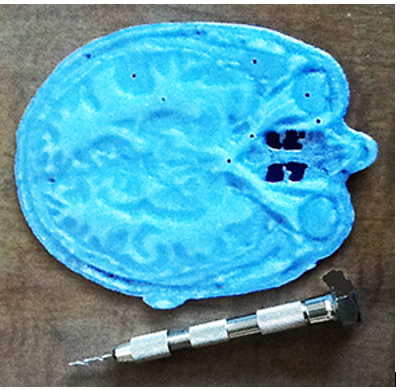
\includegraphics[width=1\linewidth]{fig 1.png}
    \caption{ 3D print of transverse section of human head showing location of drilled holes.}
    
\end{figure}

In Figure 2,The electric paint can also be applied on the tactile side far away from the drilled hole and as long as the applied electric paint forms a path to connect to the electric paint in the drilled hole, a finger touch electrical activity will be carried to the vicinity of the drilled hole and down to the iPad or iPad Pro surface.  The image in Figure 2 shows a 3D printed transverse section of the human head with a 3 cm long portion of the optic nerve covered with electric paint.  As long as the conductive electric paint touches the small hole drilled into the 3D print (see Figure 1), the charge from a fingertip touch anywhere along the optic nerve will be carried very much like a charge on an artificial wire in an electronic device down the drilled hole to the surface of the iPad or iPad Pro.  The conductive paint can also be spread over a larger brain region such as the gray matter or white matter and by connecting to just one small drilled hole filled with the same electric paint will also carry the charge of a finger touch to an audio button on an iPad or iPad Pro.  An artist’s paint brush can be used for spreading electric paint over larger areas.  But it was found that the 10 ml size of electric paint (10) from Bare Conductive comes in a tube that has a narrow nozzle for drawing circuits and it works very well for filling the small drilled hole in a 3D printed template or one drilled into a stratigraphic template made using multiple layers of 3 mm width acrylic.  As long as there is a continuous electric paint connection between the exterior surface of a 3D print or 3D laser cut template and the surface of the iPad or iPad Pro, a finger touch very efficiently causes an audio button to fire producing whatever audio is deemed important for the learning situation.

\begin{figure}
    \centering
    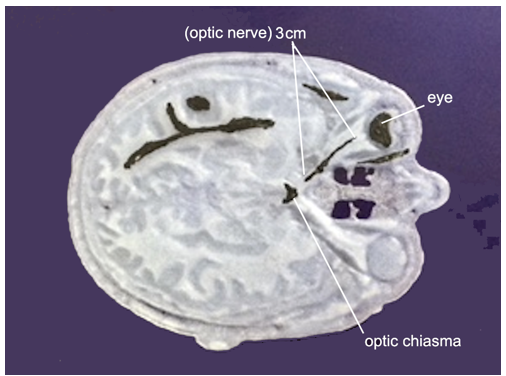
\includegraphics[width=1\linewidth]{fig 2.png}
    \caption{3D print of transverse section of human head with key structures covered with black electric paint.}
\end{figure}

\subsubsection*{iPad and iPad Pro audio-responsive software:}

The placement of audio buttons beneath the small holes filled with electric paint on a 3D laser cut template is essential for the production of information helpful to the learner.  A program titled “Hype” made by Tumult (11) is designed to produce HTML 5 animations using the Mac platform.  An image of a cell or anatomic section can be opened in Hype and importantly, Hype now permits the placement of audio buttons at any location on the screen and then permits the choice of an mp3 audio file to be linked to that button so that a touch now produces the embedded audio.  Another piece of software named NaturalReader 4.0 (12) was used to produce audio files by simply typing into NaturalReader what is desired to be made into an audio file, then select a type of voice (2 male or 2 female choices available) and now an audio file is produced.  The type of audio file produced is an aiff file but Hype only uses mp3 files so once an aiff file is made, it must be run through iTunes on the Mac to be made into an mp3 file for use by Hype in the iPad or iPad Pro environment.  The incorporation of audio files into the production of stratigraphic tactile templates expands the amount of information that can be delivered when an audio button is selected.  When all the audio buttons have been made, the Hype program is saved as an html file along with a folder containing all the important files needed for the template to respond with audio when an audio button is selected.  It is this html file that is accessed from anywhere on the Internet so that what downloads to an iPad or iPad Pro is the image complete with audio buttons that when touched will generate the audio saved on them.
      
\subsection*{Making audio-responsive tactile templates:}

The final step in the making of an audio responsive tactile template is to move and size the Hype graphic with audio buttons on an iPad or iPad Pro screen so that the audio buttons now lie directly below where the conductive paint on the template makes contact with the tablet screen.  This process takes a few moments working with both the Mac running Hype and the tactile template ready to be laid atop an iPad or iPad Pro.  Once a size modification is made using Hype on the Mac computer, the finished program is saved to a web server and now the image with audio buttons is down-loaded onto the iPad or iPad Pro.  Any needed change in size of the Hype downloaded program is determined by laying the tactile template on top of the iPad or iPad Pro screen and checking to see how well the audio buttons on the iPad and iPad Pro screen match up with the conductive paint buttons on the tactile template.  This process of sizing continues until the audio buttons in the html program produced with Hype now match where the conductive paint buttons are located on the tactile stratigraphic template.

An important difference was found between iOS 10 and iOS 11 running on the iPad or iPad Pro and the downloading of audio button html code.  In iPads running iOS 10, the audio buttons were immediately responsive to a finger touch.  In iOS 11 however, one had to access the “Action” icon (square with arrow pointing up) and then select the task named “Request Desktop Site”.  The “Request Desktop Site” downloads the full package complete with audio resources so that now the audio buttons respond when touched.  It appears that when iOS 11 and higher are running, a Hype version is downloaded that is optimized for use on a cell phone.
      
\subsubsection*{Stratigraphic Examples of audio-responsive tactile templates:}

a. Cell example I - chicken egg:  A line drawn diagram for swell paper production of a chicken egg was obtained from the TAEVIS (Tactile Access to Education for Visually Impaired Students) collection now owned by Independence Science (4).  The original chicken egg diagram was designed for use with Braille labeling to identify important regions on the chicken egg.  The Braille text and arrows were removed from the chicken egg diagram and replaced with drawings of the important regions to be identified and were then made into an svg file for use in a 3D laser cutter.  A labeled photo of the 3D laser cut chicken egg appears below in Figure 3.

\begin{figure}[h]
    \centering
    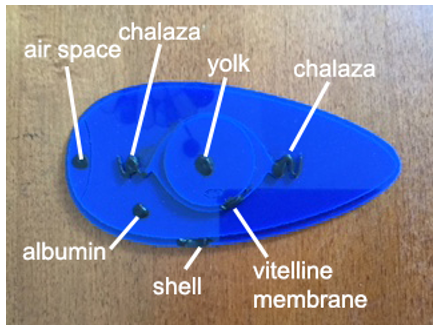
\includegraphics[width=1\linewidth]{fig 3.png}
    \caption{3D laser cut stratigraphic example of tactile template using chicken egg.}
\end{figure}
 
Figure 3, note in the image that the black areas at tip of label lines are black because they are composed of electric paint which connects to the underneath region by way of a small drilled hole also containing electric paint and this now serves as a conductive pathway to the audio button when laid atop an iPad or iPad Pro.  The above stratigraphic template is composed of four acrylic layers.  The top layer is identified as the “yolk”, the “chalaza” layer is the second layer, the “air space” and “albumin” form the third layer down from the top and the layer named the “shell” forms the bottom layer.
 
b. Cell example II - cell organelles: Another line drawn image (Image 15856) originally designed for use with swell paper to produce a tactile image was obtained from the TAEVIS collection at Independence Science and is shown in 3D laser cut form in Figure 4 below.  The layered template shows a cell and the typical organelles that many cells possess.  The original line image also contained Braille identification labels with arrows pointing to the cell organelles and structures.  The Braille and identifying arrows were removed and the completed image was made into an svg file using “Super Vectorizer 2”.  In Figure 4 below, the nucleus and many of the organelles were drawn in a form for easier tactile identification and were laser cut so that the egg itself could have the nucleus and organelles laid atop the outline of the egg in stratigraphic form as shown below.

\begin{figure}[h]
    \centering
    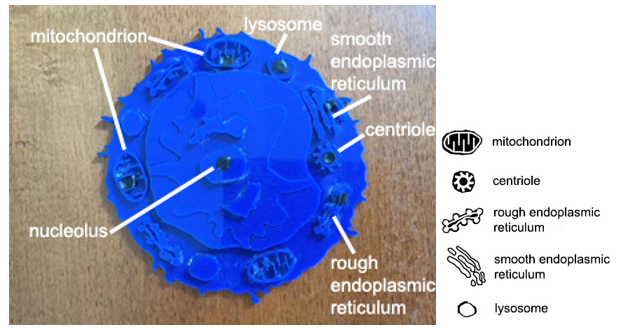
\includegraphics[width=1\linewidth]{fig 4.png}
    \caption{3D laser cut stratigraphic example of a cell and many organelles.}
\end{figure}
  
Figure 4, the Image shows a cell and five organelles identified by inserted labels and lines. An expanded view of the shape of the organelles is present to the right of the cell template to show how laser cutting can produce small pieces that are different from each other and highly tactile.  The nucleolus is the top most layer and is sitting on the nucleus (unlabeled) which forms layer two, followed by the five types of organelles on the third layer and the bottom layer is the outline of the cell so the entire cell and organelles form a four-layered stratigraphic template.  The nucleolus and organelles show black areas of conductive electric paint connecting to the hand drilled holes that can carry a finger touch electric charge to the audio buttons on the surface of an iPad or iPad Pro.
\newpage
{Figures 5a and 5b: Anatomy example - Human Left Shoulder Transverse Section \#1281 from “Visible Human” project: }
 
\begin{figure}[h] \ContinuedFloat*
   \centering
 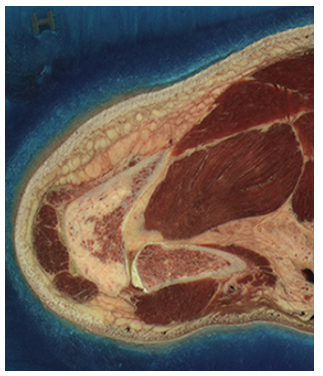
\includegraphics[width=0.5\linewidth]{fig 5a.png}
    \caption{Original transverse section \#1281 from the human left shoulder in the National Library of Medicine “Visible Human” project which was licensed for use worldwide.}
\end{figure}

\begin{figure}[h] \ContinuedFloat
       \centering
    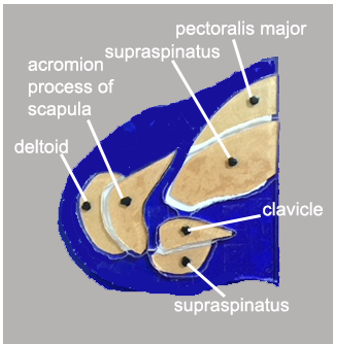
\includegraphics[width=0.7\linewidth]{fig 5b.png}
    \caption{Stratigraphic labeled shoulder joint made using the transverse section in Figure 5a.} \ContinuedFloat
\end{figure}
\newpage
Figure 5a shows the original transverse section \#1281 from the human left shoulder in the National Library of Medicine “Visible Human” project (5).  Figure 5a shows the muscles in darker red-brown color and the bones in original color making up the upper portion of the left shoulder joint.  The bone and muscle regions were outlined in black in Photoshop and made into an svg file using “Super Vectorizer 2” to make the stratigraphic labeled shoulder joint seen in Figure 5b.  Clear acrylic was used to make the muscle and bone regions.  Note the light brown color of the bones and muscles in Figure 5b which is due to the brown veneer attached to the underside of the clear acrylic pieces produced by laser cutting.  Two layers of veneer (1 mm thick wood) were attached to the underside of each of the clear acrylic pieces for the bone, i.e., the acromion process of scapula and clavicle, but only one layer of veneer was attached to the underside of the clear acrylic pieces for the muscle regions, i.e., deltoid, supraspinatus and pectoralis major.  This stratigraphic template is composed of just one layer of clear acrylic but the bone pieces have more light brown veneer layers attached to their underside surface than the muscle pieces providing a clear tactile difference when touching the template surface.  The black round areas shown on the bone and muscle acrylic pieces are the areas of added conductive electric paint that also continue through the acrylic pieces to the underside via the small hand drilled holes so that when placed on an iPad or iPad Pro, the audio buttons will then generate the name of the bone or muscle being touched.  It is also good to note that much more information can be added to an audio button than just the identity of the structure being touched as its function or even action in the case of muscles can also be included providing a platform for expanded learning and also can be designed for student testing purposes. 

Figures 6a, 6b and 6c: Human Right Shoulder Transverse Section \#1321 from “Visible Human” project”.
  
\begin{figure}[h] \ContinuedFloat*
    \centering
    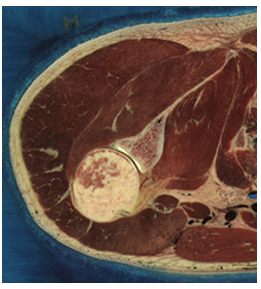
\includegraphics[width= 0.5\linewidth]{fig 6a.png}
    \caption{Original transverse section \#1321 from the human right shoulder in the National Library of Medicine “Visible Human” project which was licensed for use worldwide.}
\end{figure}


\begin{figure}[h] \ContinuedFloat
    \centering
    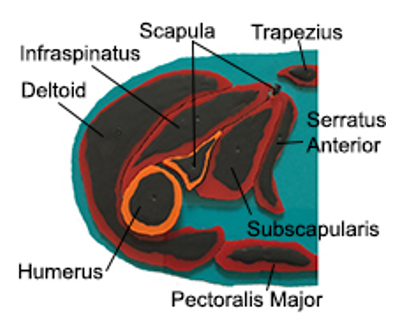
\includegraphics[width=1\linewidth]{fig 6b.png}
    \caption{ A stratigraphic labeled shoulder joint using the transverse section in Figure 6a.}
\end{figure}

\newpage
In Figure 6a, the bone and muscle regions were outlined in black in Photoshop and made into an svg file using “Super Vectorizer 2” to make the stratigraphic labeled shoulder joint seen in Figure 6b.  Small holes were hand drilled into the bone and muscle regions, filled with conductive electric paint and a large area of the top surface for each muscle and bone region was covered with conductive electric paint.  Text and lines were added to label the bone sections (head of humerus, scapula and a small portion of the shoulder blade) and the muscle regions (deltoid, infraspinatus, supraspinatus, pectoralis major and trapezius).  This template can be laid atop an iPad or iPad Pro with an image of the right shoulder joint section with audio buttons just under the muscle or bone regions so that when the upper layer is touched, the audio button underneath the template will fire with the muscle or bone name.  Note that the conductive filament covers a wide area of the muscle or bone regions and a touch at any spot will carry the finger electric charge to the small drilled hole filled with electric paint and down to the audio button on the iPad or iPad Pro surface. 

\begin{figure}[h] \ContinuedFloat
    \centering
    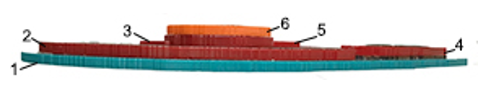
\includegraphics[width=1\linewidth]{fig 6c.png}
    \caption{side view of the stratigraphic labeled shoulder joint shown in Figure 6b.}
    
\end{figure}

Note in Figure 6c, the muscle and bone layers are identified by their tactile position from bottom to top.  Layer 1 at bottom is the skin and fascia made from a single 3 mm acrylic piece, layer 2 is a single 3 mm acrylic piece to indicate position of the deltoid muscle.  Layer 3 represents the infraspinatus and is composed of a 3 mm acrylic piece and one layer of 1 mm veneer (4 mm height), Layer 4 is the pectoralis major composed of one 3 mm acrylic piece and one I mm veneer piece for a total of 4 mm,  layer 5 is the subscapularis composed of one 3 mm acrylic piece and two 1 mm veneer pieces for total of 5 mm and layer 6 is the humerus and scapula made from three 3 mm acrylic pieces for a tactile height of 9 mm.  The pectoralis major muscle, \#4 in Figure 6c, is composed of one 3 mm acrylic piece and one 1 mm veneer piece for a total of 4 mm as it is next to the deltoid muscle which is made of a single 3 mm acrylic piece.  The trapezius is not touching another muscle in this section and is a single 3 mm acrylic piece.  Figure 6c shows how the combination of stratigraphic layering with both 3 mm acrylic pieces and 1 mm thick veneer can provide a wide variation of tactile options so that muscles and/or bones that lie next to each other can be differentiated and identified in a stratigraphic way in a touch sensitive audio-responsive template. 

\section*{SUMMARY}
This report demonstrates a role for 3D laser cutting techniques when combined with stratigraphic methods and use of electric paint in the production of audio-responsive tactile templates in the study of STEM material by students who may be blind.  Although this study focused on microscopic and anatomic subjects in the fields of biology and anatomy, the use of stratigraphic methods, electric paint and 3D laser cutting can be seen as useful for other science disciplines as well.  The 3D tactile templates studied in this report appear quite robust and can weather rough handling so should last a long time in terms of their productive usage.  There are several repositories of STEM images available for making stratigraphic audio templates such as the NIH 3D Print Exchange (13) where the author has contributed stl files for the 3D printing of the stages of mitosis (14), the National Library of Medicine Visible Human project (5) and with permission the Bassett Collection of anatomic images (15), the APH Tactile Image Library (16), NASA 3D Resources (17) and some STEM files in Thingiverse (18).  None of these repositories have files designed specifically for making into stratigraphic audio-responsive templates so the field is wide open for exploring which files may be best modified to meet the needs for learning STEM by blind students.  3D laser cutting methods are not intended as a replacement for all raised line graphics or 3D printed tactile templates but should be viewed as another option to consider when decisions are made about which templates are to be designed for study.

The examples of 3D laser cut stratigraphic templates shown in this report await rigorous testing and the author will gladly share these examples and others designed for STEM learning for testing purposes and if desired, will be happy to assist in the production of more templates for testing.


\end{large}
\clearpage
\section*{REFERENCES}\par 

\leftskip 0.25in
\parindent -0.25in 
Kolitsky, Michael A, 3D printing makes virtual world more real for blind learners, e-Mentor 2016, number 1 (63) at \url{http://www.e-mentor.edu.pl/artykul/index/numer/63/id/1222}

\url{https://www.bareconductive.com/}

\url{https://glowforge.com/}

\url{http://independencescience.com/}

\url{https://www.nlm.nih.gov/research/visible/visible\_human.html}

\url{https://www.bareconductive.com/}

Kolitsky, Michael A., 3D Printed Tactile Learning Objects: Proof of Concept, Journal of Blindness Innovation and Research 2016, Vol 4, No 1, \url{https://nfb.org/images/nfb/publications/jbir/jbir14/jbir040102.html}

\url{https://glowforge.com/customer-gallery}

\url{http://www.svgvector.com/vectorize-imagemac.html}

\url{https://glowforge.com/m/proofgrade}

\url{https://www.bareconductive.com/shop/electric-paint-10ml/}

\url{https://tumult.com/hype/}

\url{https://www.naturalreaders.com/}

\url{https://3dprint.nih.gov/}

\url{https://3dprint.nih.gov/discover/3dpx-000519}

\url{http://lane.stanford.edu/biomed-resources/bassett/raw/index.html}

\url{https://www.aph.org/tgil/}

\url{https://nasa3d.arc.nasa.gov/models/printable}

\url{https://www.thingiverse.com/}
\end{document}